% !TeX encoding = UTF-8
\documentclass[12pt,utf8]{beamer}
\usepackage{graphicx}
\usepackage{xcolor}
\usepackage[ngerman]{babel}
\usepackage{wasysym}
\input{Latex_Template/beamerthemeFOSSAG.sty}

\title{Shells}
\subtitle{Alternativen zu Bash}
\author[Free and Open Source Software AG]{Nicolas Lenz}
\institute[FOSS AG]{Free and Open Source Software AG\\Fakultät für Informatik}
\date{\today}

\begin{document}
    \begin{frame}
    \titlepage
\end{frame}

\begin{frame}
    \frametitle{Inhalt}
    \begin{itemize}
        \item Einleitung
        \item Die Anfänge
        \begin{itemize}
            \item Thompson-Shell
            \item Bourne-Shell
            \item C-Shell
            \item Korn-Shell
        \end{itemize}
        \pause
        \item Shell-Vielfalt
        \begin{itemize}
            \item Bourne-Again-Shell
            \item BusyBox
            \item Debian-Almquist-Shell
        \end{itemize}
        \pause
        \item Live-Test
        \begin{itemize}
            \item Z-Shell
            \item Friendly Interactive Shell
        \end{itemize}
    \end{itemize}
\end{frame}

\begin{frame}
    \frametitle{Einleitung}
    \begin{itemize}
        \item Bisher haben wir nur die bash als Shell benutzt
        \item Vielfältige Auswahl an Shells für verschiedene Einsatzbereiche
        \item Unterscheiden zwischen der Shell-Skriptsprache und dem interaktiven Modus
    \end{itemize}
\end{frame}

    \begin{frame}
    \frametitle{Die Thompson-Shell}
    \begin{itemize}
        \item Heute bekannt als \textbf{``osh``} für ``old shell``
        \item Verwendet in den ersten Versionen von \textbf{UNIX} seit \textbf{1971} (vor 46 Jahren)
        \item Führte Piping, einfache Kontrollstrukturen für Skripte und Wildcarding ein
    \end{itemize}
\end{frame}

\begin{frame}
    \frametitle{Die Bourne-Shell}
    \begin{itemize}
        \item Ursprünglich veröffentlicht \textbf{1977} (vor 40 Jahren)
        \item Heute bekannt und immer noch genutzt als \textbf{``sh``}
        \item Führte \textbf{Umgebungsvariablen} ein
        \item Erweiterte die Skriptfähigkeiten und führte heutige Syntax ein
        \begin{itemize}
            \item Inspiriert von \textbf{ALGOL68}
            \item Bspw. \textbf{if} mit \textit{if} und \textit{fi} und \textbf{switch} mit \textit{case} und \textit{esac}
        \end{itemize}
        \item Skript-Syntax mittleweile in POSIX standardisiert
    \end{itemize}
\end{frame}

\begin{frame}
    \frametitle{Die C-Shell}
    \begin{itemize}
        \item Erschienen \textbf{1978} (vor 39 Jahren), also kurz nach der Bourne-Shell
        \item Kurz \textbf{``csh``}
        \item Andere Skriptsyntax als die \textbf{sh}
        \begin{itemize}
            \item Inspiriert von \textbf{C}
            \item Konnte sich aber nicht durchsetzen
        \end{itemize}
        \item Führte viele wichtige Funktionen für den \textbf{interaktiven Modus} ein
        \begin{itemize}
            \item Verlauf
            \item Aliase
            \item Dateinamen-Vervollständigung
        \end{itemize}
    \end{itemize}
\end{frame}

    \begin{frame}
    \frametitle{Die Bourne-Again-Shell}
    
\includegraphics[height=1.2cm]{res/bash.png}
    \begin{itemize}
        \item Veröffentlicht \textbf{1989} (vor 28 Jahren)
        \item Nachfolger der Bourne-Shell (daher der Name)
        \item Kurz \textbf{bash}
        \item Kombiniert Skript-Syntax der \textbf{sh} mit den interaktiven Funktionen der \textbf{csh}
        \item Heute der Standard unter \textbf{Linux} und \textbf{macOS}
    \end{itemize}
\end{frame}

\begin{frame}
    \frametitle{BusyBox}
    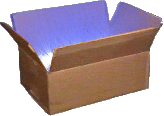
\includegraphics[height=1.2cm]{res/busybox.png}
    \begin{itemize}
        \item Mehr als eine Shell
        \item Viele sonst selbständige Tools in einer \textbf{einzigen Datei}
        \begin{itemize}
            \item ls
            \item cat
            \item grep
        \end{itemize}
        \item Dadurch weniger Overhead
        \item Beliebt im Embedded-Bereich und z.B. als Notfall-Shell
    \end{itemize}
\end{frame}

\begin{frame}
    \frametitle{Debian-Almquist-Shell}
    \begin{itemize}
        \item \textbf{dash} - Verbesserung der Almquist-Shell (\textbf{ash}) für die Debian-Linux-Distribution
        \item Leichtgewichtig
        \item In Debian und Ubuntu daher Standard für Skript-Ausführung
        \item Im Embedded-Bereich beliebt
    \end{itemize}
\end{frame}

\begin{frame}
    \frametitle{PowerShell}
    
\includegraphics[height=1.2cm]{res/powershell.png}
    \begin{itemize}
        \item \textbf{2006} entwickelt von Microsoft
        \item Ersatz für die alte und sehr leistungsschwache cmd.exe
        \item Funktionsreiche Skriptsprache basierend auf .NET
        \item Open-Source und auch unter Linux nutzbar
    \end{itemize}
\end{frame}

\end{document}
